%*******************************************************************************
%****************************** Second Chapter *********************************
%*******************************************************************************

\chapter{Data Stream Model(10 pages)}

\ifpdf
    \graphicspath{{Chapter2/Figs/Raster/}{Chapter2/Figs/PDF/}{Chapter2/Figs/}}
\else
    \graphicspath{{Chapter2/Figs/Vector/}{Chapter2/Figs/}}
\fi

% Time
% Tuple
% Data Stream

\subsection*{Order}
Ordering is rather important in Distributed system, specially Stream Processing System in particular. 

In traditional model, there are a single program, one process, one memory space running on one CPU. Programs are written to be executed in an ordered fashion in queue:  staring from the beginning, and then going  toward the last. In distributed system, programs run in many machines across the network but try to reserve the order of the result. One of easiest way to define "correctness" is to say "it works like it would on a single machine". And that usually means that a) we run the same operations and b) that we run them in the same order - even if there are multiple machines. \citep{Mikito:2014}

In theory, they are defined 2 types of orders: total order and partial order. 

\begin{defi}
 Paritial order is a binary relation $\leq$ over a set $P$ which is reflexive, anti-symmetric and transitive, i.e., which satisfies for all $a$, $b$ and $c$ in $S$ (wiki):
 
 \begin{itemize}
	 \item $a \leq a$ (reflexivity)
	\item  if $a \leq b$ and $b \leq a$ then $a = b$ (antisymmetry) 
	\item if $a \leq b$ and $b \leq c$ then $a \leq c$  (transitivity)
\end{itemize}
\end{defi}

\begin{defi}
 Total order is a binary relation ``$\leq$'' over a set $S$ which is anti-symmetric and transitive and total. Therefore, total order is a partial order with totality
 
 \begin{itemize}
	 \item $a \leq b$ or $b \leq a$  (totality)
\end{itemize}
\end{defi}

Total order ``<'' is strict on a set $S$ if and only if $(S, <)$ has no non-comparable pairs:
\begin{equation}
 \forall x, y \in S \Rightarrow  x < y \cup y < x 
\end{equation} 

In a totally ordered set, every two elements are comparable whereas in a partial ordered set, some pairs of elements are incomparable and hence we do not have the exact order of every item.

The natural state in a distributed system is partial order. Neither the network nor independent nodes make any guarantees about relative order; but at each node, you can observe a local order.

In streaming processing, one may discretize a stream into a discrete stream of windows. Therefore, we need to specify the order of elements to define which elements should be inserted into a given window. Furthermore, data stream involve the temporal order and the positional order \citep{Petit:2012} in stream. 

The \textbf{temporal order} is induced by the timestamp of items in a stream. Using the value of timestamp, one can determine whether something happen chronologically before something else. Nevertheless, if some items happen simultaneously, they will have the same timestamp, then it may not be strict. For instance, there are two items with the same timestamp but system is required to take one only, the chosen is non-deterministic between two. Therefore, we may require a strict order.

The \textbf{positional order} is a strict order induced by the position of items in stream. Two items  may have the same timestamp but one may arrive before the other so that they have different positional orders. The positional order can be defined by arrival order or id of item regardless of explicit timestamp. 


//TODO:The temporal order: Order. When I say that time is a source of order, what I mean is that:

we can attach timestamps to unordered events to order them
we can use timestamps to enforce a specific ordering of operations or the delivery of messages (for example, by delaying an operation if it arrives out of order)
we can use the value of a timestamp to determine whether something happened chronologically before something else.

\subsection*{Time}
\textbf{Time Domain} The time domain $\mathbb{T}$ is a discrete, total ordered, countably infinite set of time instants $t \in \mathbb{T}$. We assume that $\mathbb{T}$ is bounded in the past , but not necessarily in the future. For the sake of simplicity, we will assume that the time domain is the domain of non-negative long integer ($\mathbb{T} = \mathbb{N}$) {0,1,2,3,..}\citep{Dindar:2013} and totally ordered. 

2 type of times: system time $t^{sys}$ (implicit) and application time $t^{app}$ (explicit). These both take values from the time domain $\mathbb{T}$, but carry two different meaning. 

\textbf{Application Timestamps} In many case, each item in stream contains an explicit source-assigned timestamp itself. In other words, the timestamp attribute will be a part of the stream schema. Consider  a common log format for web application which contains a timestamp specifying when the action is taken place. 
A log line record user named \textit{pablo} to get an image
\begin{verbatim}
216.58.209.174 user-identifier pablo [10/Oct/2000:13:55:36 -0700] \\
"GET /image.gif HTTP/1.0" 200 1234
\end{verbatim}
Sequence number attribute could represent a timestamp instead.

\textbf{System Timestamps} Even if the item arrives at the system are not equipped with a timestamp, the system assigns a timestamp to each tuple, by default using the system’s local clock. While this process generates a raw stream with system timestamps that can be processed like a regular raw stream with application timestamps, the user should be aware that application time and system time are not necessarily synchronized\citep{Kramer:2009}. Since system timestamp is assigned implicitly by system , one may not notice it presence on schema. As we mentions above, time domain is total ordered in local machine , but partial ordered across the system because of possible postpone on processing or asynchronous timestamp at different node.


Both application and system timestamp captures time information but they cary two different meanings. The former is related to the occurrence of the application event( when the event happens), whereas the latter is related to the occurrence of related system(when the corresponding event data arrive at system). Multiple items may have the same application timestamps but they will not arrive in the same order. Therefore, system will assign the different unique system timestamp based on their arrival. Sytem then can believe in the system timestamp as a strict total ordered basis for reasoning about arrival items to perform processing. For example, another log from different users arrive at system:
\begin{verbatim}
219.53.210.143 user-identifier fabio [10/Oct/2000:13:55:36 -0700] \\
"GET /image.gif HTTP/1.0" 200 1432
\end{verbatim}
However, it might arrive after the first log for user \textit{pablo} then system would response \textit{pablo}'s first, instead of \textit{fabio}'s request.

\textbf{Note}: more on Timestamp in Streams \citep{Babcock:2002} page 13

\subsection*{Tuple}
A tuple is a finite sequence of atomic values. Each tuple can be defined by a Schema corresponding to a composite type. Tuple can represend a relational tuple , a event or a record of sensor data and so on. \citep{Arasu:2006:CCQ}. For instance, the log format in previous example follow a schema:

\begin{verbatim}
<SourceIP, IdentityType, user, timestamp, action, response, packageSize >
\end{verbatim}

A data tuple is the fundamental, or atomic data item, embedded in a data stream and processed by an application. A tuple is similar to a database row in that it has a set of named and typed attributes. Each instance of an attribute is associated with a value\citep{Henrique:2014}. Furthermore, one can consider a tuple as a partial order mapping a finite subset of attribute names to atomic values\citep{Petit:2012}. A tuple consits of a set of (Atribute x Value) pairs such as $(SourceIP, 219.53.210.143)$



\section{Stream Model}


Based on time and tuple domain, basically, CQL \citep{Arasu:2006:CCQ} defines a data stream as
\begin{defi}
	A stream $\mathbb{S}$ is a countably continuous and infinite set of elements $<s,t> \in \mathbb{S}$, where $s$ is a tuple belonging to the schema of $\mathbb{S}$ and $t \in \mathbb{T}$ is the timestamp of the element. 
\end{defi}

There are several stream definitions varying based on the execution model of systems. On the previous definition, a timestamp attribute can be an non-strict total ordered application timestamp so that system may not rely on it to order the coming tuples to react on them. For this reason, stream can contain an extra physical identifier  $\varphi$ \citep{Petit:2010} such as increment tuple id to specify its order. The tuple with smaller id mean that they arrive and should be processed before the tuples with bigger id. Another way to identify the order of a tuple item is to separate the concept of application and system timestamp. In SECRET model \citep{Botan:2010}, each stream item is composed of a tuple for event contents , an application timestamp, a system timestamp, and a batch-id value. The idea of batch-id is critical to SECRET system we do not mention in the thesis.
In short, in practice, we assume that elements of a stream are totally ordered by the system timestamp and physical identifier.

In Apache Flink, for the flexibility, system accepts a user-defined timestamp function   $f: \mathbb{TP} \rightarrow \mathbb{T}$ to map a tuple to its application timestamp value. One of the most common scenario is that the function $f$ extract one attribute of Schema and consider it as timestamp value.

Consider the example of temperature sensors, the sensors feed a stream $S(TIME\ :\ long,TEMP:\ int)$ indicating that at the \textit{TIME}, the temperature is \textit{TEMP}. Since $TIME$ attribute has the $long$ long, we are able to consider it as a timestamp due to function
\begin{equation}
f: (TIME, TEMP) \rightarrow SEC
\end{equation}

However, we may receive the stream from a different timezone. Thus, the application timestamp must be converted to the current timezone for the sake of data integration. For instance, one acquires the timestamp value (in milliseconds) in next timeszone.
\begin{equation}
f: (TIME, TEMP) \rightarrow TIME + 3600*1000
\end{equation}


I propose the definition of Stream $s:<v>$ extends to $s:<v, t_{app}, t_{sys}>$, with $t_{app} = f(v)$ , $t_{app} \in \mathbb{T}$, $t_{sys} \in \mathbb{T}$

For further analysis on execution model in Apache Flink, I propose a extend definition of a data stream as:

\begin{defi}
	A stream $\mathbb{S}$ is a countably infinite set of elements $s \in \mathbb{S}$. Each  stream element $s: <v, t_{app}, t_{sys}>$, consists of a relational tuple v conforming to a schema $TP$, with an \textit{optional} application time value $t_{app} = f(v) \in \mathbb{T}$, and a timestamp $t_{sys}$ generated automatically by system, due to the event arrival.
\end{defi}
With the partial function $f$ to extract application timestamp from tuple: $f: \mathbb{TP} \rightarrow \mathbb{T}$


 
\subsection*{Data Stream Properties} 
In the data stream model, some of all the input data that are to be operated are not available for random access from disk or memory, but rather arrive as one or more continuous data streams. Data streams differ from the conventional stored relation model in several ways\citep{Babcock:2002}


Data Stream may have the following properties \citep{Golab:2010}:
\begin{itemize}
	\item They are considered as sequences of records, ordered by arrival time or by another ordered attributed such as generation time which is explicitly specified in schema, that arrive for processing over time instead of being available a priori. Totally order by time. 
	\item They are emitted by a variety of external sources. Therefore, the system has no control over the arrival order or data rate, either within a stream or across multiple streams
	\item They are produced continually and, therefore, have unbounded, or at least unknown, length. Thus, a DSMS may not know if or when the stream "ends". We may set a time-out waiting for new event. Exceeding the time-out, the stream considerably ends. 
	\item Typically, big volume of data arrives at very high speed so that data need to process on the fly. Once an element from a data stream model has been processed it is discarded or archived. Stream elements cannot be retrieved, unless it is explicitly stored in storage or memory, which typically is small relative to the size of the data stream. \citep{Babcock:2002}
	
\end{itemize}


\subsection*{Stream Representations}
\subsubsection*{Base Stream vs. Derived Stream}
We distinguish 2 kinds of streams: \textit{base stream}(source stream) and \textit{derived stream}. Base stream stream is produced by the sources whereas derived stream is produced by continuous queries and their operators\citep{Arasu:2006:CCQ}. For example, \citep{Golab:2010} page 17
From now on, we give example queries on input stream named \textit{StockTick}\citep{StreamBaseTut} and the schema associated with the incoming tuples includes 4 fields:
\begin{itemize}
\item \textbf{Symbol}, a string field of maximum length 25 characters that contains the symbol for a stock being traded (e.g. IBM);
\item \textbf{SourceTimestamp}, a timestamp field containing the time at which the tuple was generated by the source application(timestamp is represented with date time format or long integer);
\item \textbf{Price}, a double field containing transaction price
\item \textbf{Quantity}, a integer fields that contains the transaction volume
\item \textbf{Exchange}, a string field of maximum length 4 that contains the name of Exchange the trade occurred on (e.g. NYSE)

\end{itemize}
A sample tuple represents the price of IBM stock unit is 81.37 at ``1 May 2015 10:18:23" from NYSE market 
\begin{verbatim}
<IBM,1430468303,81.37,NYSE>
\end{verbatim}

The \textit{StockTick} is emitted directly from source so that it is a base stream. However, a below \textit{HighStockTick} stream is a derived stream originated from \textit{StockTick}. \textit{HighStockTick} contains only transaction of stock with price of more than \$100 each unit.

\begin{verbatim}
CREATE STREAM HighStockTick AS
	SELECT * FROM StockTick 
	WHERE price > 100
\end{verbatim}

In practice, base stream are almost always append-only , mean that previously arrived stream elements are never modified. However, derived stream may or may not be append-only\cite{Golab:2010}. A derived stream that present the average transaction volumes between interval time $[t_1, t_2]$. The query produce an element $s_1$ to the stream immediately after $t_2$. However, an element of \textit{StockTick} stream with timestamp 
$t_{12} \in [t_1,t_2]$ arrive late at $t_2+\phi$. If the system takes into account of the late arrival element, it will update the previous average volumes at $[t_1, t_2]$. In this case, this derived stream is not append-only.


\textbf{Note}: another examples from \textbf{epl-guide}
\textbf{Note}: stock example : http://www.codeproject.com/Articles/553206/An-Introduction-to-Real-Time-Stock-Market-Data-Pro


\subsubsection*{Logical Stream vs. Physical Stream}
Logical stream ?  \citep{Kramer:2009}Physical stream ?  \citep{Kramer:2009}

Logical stream is a conceptual and abstract data stream which is processed linearly through a series of chaining operators. According to logical data flow graph, one is able to observe the order of operators that data is processed and what are the input and output of process.

Physical stream flow graph indicates how system really process the data in data parallelism environment. Physical operator is replicated and the internal operator state is partitioned and segmented. Figure~\ref{fig:streamRepresent} depict the different between logical and physical data flow.
A logical stream from source go straight through an aggregate and a filter operator before written to Sink, whereas physical streams are segmented and go through different internal replica of the same logical operator. Eventually, all physical streams will be merged and written to one Sink. 

%\begin{wrapfigure}{l}{0.7\textwidth} 
 %   \centering
  %  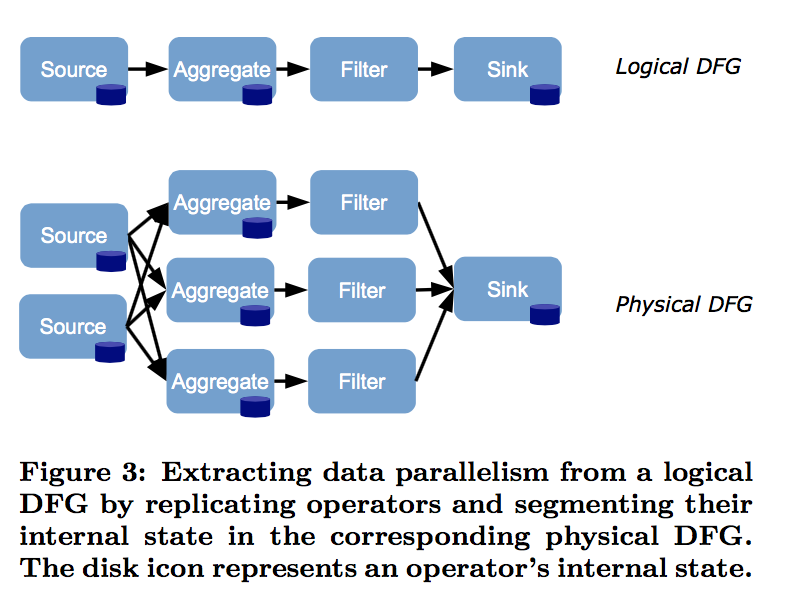
\includegraphics[width=0.7\textwidth]{logicalPhysicalDataFlow}
%\caption[Minion]{Stream Processing in Action. Henrique Andrade}
%\label{fig:streamRepresent}
%\end{wrapfigure}

\begin{figure}[htbp!] 
\centering    
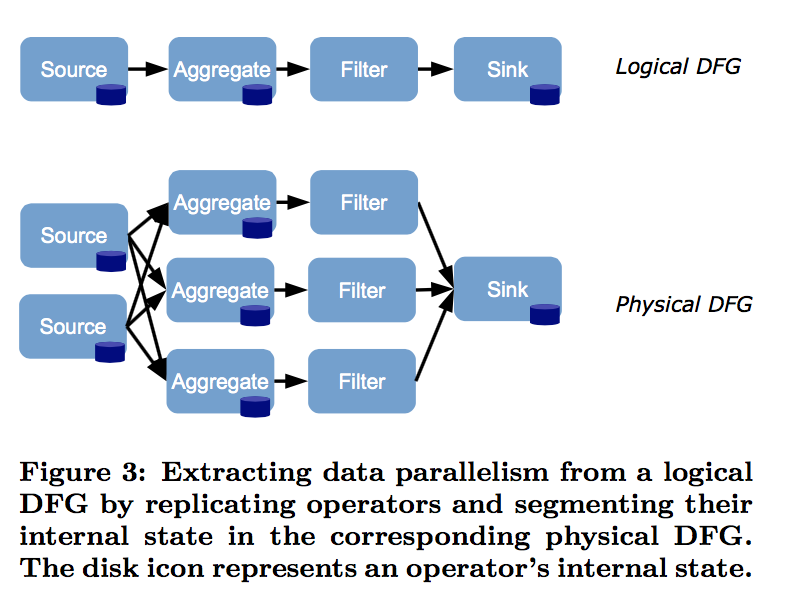
\includegraphics[width=0.7\textwidth]{logicalPhysicalDataFlow}
\caption[Minion]{Stream Processing in Action. Henrique Andrade\citep{Henrique:2013}}
\label{fig:streamRepresent}
\end{figure}

   
\subsection*{Signals[Option]}    \citep{Golab:2010} 
    
    
\section{Stream Windows}

Why do we need window?

From the system's point of view, it is often infeasible to maintain the entire history of the input data stream. Because data stream is running infinitely, we do not know when it ends. It nearly impossible to query over the entire stream with some operators such as sum, average. Accumulating a tuple attribute for entire stream may results to a very big value causing  buffer overflow. From the user's point of view, recently data may be insight and more useful to make a data-driven decision. Those reasons motivated the user of windows to restrict to the scope of continuous queries. 

Many stateful stream processing operators are designed to work on windows of tuples, making it a fundamental concept in stream processing. Therefore, a stream processing language must have rich windowing semantics to support the large diversity in how SPAs can consume data on a continuous basis.

\begin{defi}
A \textbf{Window} $W$ over a stream $\mathbb{S}$ is a finite subset of stream $\mathbb{S}$ \cite{Dindar:2013}
\end{defi}


A window over streaming data can be created, buffering a continuous sequence of individual tuples. However, the size of window is a finite number so that system must decide what and how to buffer data based on the window specification. 

The specification consists of several parameters :
\begin{enumerate}
\item an optional partitioning clause, which partitions data in window into several groups. Query on window will be taken place regard for each group, instead of the whole window
\item a window size, that may be expressed either as the number of tuples included in it or as the temporal interval spanning its contents
\item an optional window slide, the distance between the starts of 2 consecutive window (i.e., waiting 2 seconds or 5 data elements before starting a new window). This crucial property determine whether and in what way a window change state over time.
\item an optional filtering predicate, keeping only elements that satisfy the predicate.
\end{enumerate}

//Example : 


Windows can be construct according to (window specification) that define what to buffer, resulting in many window variations. These variations differ in their policies with respect to evicting old data that should no longer be buffered, as well as in when to process the data that is already in the window.\citep{Henrique:2014}



Window may be classified according the following criteria:

\subsection{Direction of movement}
Window can fixed or sliding along the stream.
\begin{itemize}

\item Fixed Window:  has both upper-bound and lower-bound fixed. Therefore the window is evaluated only once and capture a constant portion information of stream

Example: //TODO

\item Sliding window: the width of the window may be fixed in term of logical unit (i.e., time interval units) or physical unit (i.e., tuple count in window). However, the boundaries of windows change overtime along the stream.

Example: //TODO

\item Tumbling window: a particular sliding window where the boundaries move is equal to the window's width. Windows are disjoint.

Example: //TODO

\item Landmark Window: One of the bounds remains  anchored at a specific system timestamp. The other edge of the window is allowed to move freely. Usually, the lower-bound is fixed , and the upper-bound shifted forward in pace with time progression

\end{itemize}


\subsection{Definition of contents} time-based, count-based/tuple-based, partitioned windows, predicate window

\begin{itemize}
	\item Logical or time-based windows are defined in terms of time interval, e.g., a time-base sliding window may maintain the the last one minutes of data.
	
	\item Physical(also known as count-based or tuple-based) windows are defined in terms of the number of tuples, e.g., a count-based window sliding window may store the last arrived 100 tuples.
	
	\item Delta-based windows are defined in terms of a delta function and a threshold value. The function calculates a delta between 2 elements such as absolute distance or Euclidean distance between 2 data elements. In delta-based windows, the delta between the first element and any of the rest must not be larger than the threshold, respectively.For example, assuming that window satisfies the euclidean distance between the first and other element is not higher than 10. Currently arrival data point will join the window if the delta between it and the first elements of window is equal or less than threshold. Otherwise, the window is closed and emitted; the currently arrival data point trigger a new window. Formally, a delta windows contains $n$ ordered elements $a_1, a_2,...,a_n$ so that every elements $a_k$ with $k \in [1,n]$ must satisfies
	\begin{equation}
		\Delta(a_1,a_k) \leq \phi
	\end{equation}

	\item Partitioned Windows contain only the elements  in the same group which differentiates itself from the other groups  by the value of a grouping attributes (subset of its schema), e.g., a partitioned window store last 100 elements with the same value of (\textit{StockSymbol}, \textit{Exchange}). Thus, several  substreams are derived logically from the real stream, each one corresponding to an existing combinations of value$<a_1,a_2,...,a_k>$ on the grouping attributes. Each group maintains a separate window buffer to capture arrival events and emit when satisfies window specification.
	
	
	\item Predicate window \citep{Ghanem:2008} , in which an arbitrary logical predicate specifies the contents. Only data point that satisfies the predicate will join the window, otherwise it is discarded. e.g.,predicate window maintain last 100 transactions have more than 100.000 units in terms of \textit{volume}.
	
\end{itemize}

%\subsection{Frequency of movement[Optional]} jumping window, mixed jumping window, tumbling window

%By default, a time-based window is updated at every time tick, and a count-based window is updated when a new tuple arrives. A jumping window is updated every k ticks or after every kth arrival. Note that a count-based window may be updated periodically, and a time-based window may be updated after some number of new tuples have arrived; these are referred to as mixed jumping windows [Ma et al., 2005]. If k is equal to the window size, then the result is a series of non-overlapping tumbling windows [Abadi et al., 2003].
%In practice, tumbling windows, such as the one-minute windows in query Q1 from Sec- tion 2.1.1, are popular due to the simplicity of their implementation—at the end of each window, the query resets its state and starts over. Forward-sliding windows (time-based and count-based) are also appealing due to their intuitive semantics, especially with joins and aggregation, as we will discuss below. However, sliding windows are more difficult to implement than tumbling windows; over time, a continuous query must insert new tuples into a window and remove expired tuples that have fallen out of the window range.


(check Sliding Window Query Processing over Data Stream pages 25)


The notion of sliding windows requires at least an ordering on data stream elements. In many cases, the arrival orders of the elements suffices as an \"implicit timestamp\" attached to each data element. However, sometimes it is preferable to user \"explicit timestamp\" provided as part of data stream. Formally, we say that a data stream consists of a set of (tuple, timestamp) pairs. Timestamp attribute could be a traditional timestamp or it could be a sequence number - all that is required is that it come from a totally ordered domain with a distance metric. The ordering induced by the timestamp is used when selecting the data elements making up a sliding window. 


\textbf{Notes}: in CQL tuple-based sliding window may be non-deterministic - and therefore may not be appropriate - when timestamp are not unique

\textbf{Notes}: Streambase: tuple-at-a-time

\textbf{Notes}: Tuple relational calculus by Edgar F. Codd

\textbf{Notes}: \href{http://en.wikipedia.org/wiki/Relational\_algebra}{http://en.wikipedia.org/wiki/Relational\_algebra}

